\chapter{Experiments and Results}
\label{chapter:experiments-and-results}

This Chapter describes a series of experiments that were performed in order to
demonstrate the capabilities of the proposed method regarding two areas:
forecasting and interpretability. The forecasting capabilities of the method are
demonstrated by exhibiting how the multi-agent model simulates the prices in
training and testing datasets, and how the system's curve-fitting error
decreased throughout the genetic algorithm's generations. The simulated profits
are also included, for both the training and testing datasets. These plots along
with some discussions of the results are provided in Section
\ref{section:forecasting-the-prices-of-a-financial-market}. Regarding the
interpretation capabilities of the method, a description of how the agents
perceive the market is shown. This description also describes what actions the
agents take according to their perceptions. These interpretations can be found
in Section \ref{section:extracting-insights-about-a-financial-market}, along
with their respective discussions.

All of the experiments were optimized for a total of 100 generations. The reason
behind this is that the number of experiments was relatively big for this
thesis document because of the combinations among the number of markets, number
of agents, number of rules and number of individuals. Additionally, some
undocumented experiments were showing a stagnation after the 100th generation
regarding error minimization.

The experiments cover the following variants in the parameters: 4 agents, 4
rules and 4 individuals; 10 agents, 10 rules and 10 individuals; 20 agents, 20
rules and 20 individuals; and these variants are used to created models for the
following foreign exchange markets: AUD/USD, EUR/GBP, EUR/USD, GBP/USD and
USD/CAD.

A total of 135 experiments were performed, but due to space constraints in this
thesis document, only some of the experiments are shown. Specifically, the
forecasting and interpretation Sections show results for the cases of 4 agents,
4 rules and 4 individuals; 10 agents, 10 rules and 10 individuals; and 20
agents, 20 rules and 20 individuals. Each of the aforementioned cases are
extracted for each of the five foreign exchange markets: AUD/USD, EUR/GBP,
EUR/USD, GBP/USD and USD/CAD. The reader can find the plots and interpretations
for all the experiments performed in the Git repository of this thesis here:
https://github.com/amherag/PhD-Thesis/.

\section{Forecasting the Prices of a Financial Market}
\label{section:forecasting-the-prices-of-a-financial-market}

This Section shows some experiments that have the goal of forecasting different
foreign exchange markets. Different agent-based models were generated using the
parameters indicated in each of the Subsection titles. The datasets used for the
training stage of the model comprehends the prices and timestamps associated to
each of these prices, from Monday, January 28, 2019 5:00:00 PM GMT-08:00, minus
20 hours that are required to generate the initial retracements (see Section
\ref{section:preprocessing-a-financial-market-using-retracements:implementation})
to Sunday, February 3, 2019 8:00:00 PM GMT-08:00. Regarding the datasets used
for the testing stage of the model, the data comprehends the prices and
timestamps associated to each of these prices, from Sunday, February 3, 2019
9:00:00 PM GMT-08:00, minus 20 hours that are required to generate the initial
retracements, to Friday, February 8, 2019 12:00:00 AM GMT-08:00. All the
datasets have a size of 100 data points, and they correspond to the prices of
the foreign exchange markets AUD/USD, EUR/GBP, EUR/USD, GBP/USD and USD/CAD
according to the corresponding experiments Section.

Each of the following Subsections shows five plots: two plots of the
curve-fitting of the optimized model for the training and testing datasets, two
plots of the profits generated by the simulated trades of the optimized models
for the training and testing datasets, and a plot of the error minimization in
the training or optimization stage. The titles of the plots for both the
training and testing stages also include the mean-squared error in parentheses
(denoted by $\epsilon$) for the simulated versus real prices. The profit plots
show the accumulated profits through time in asset units. The minimization plot
shows the mean-squared error obtained by the best individual in each of the
generations.

\newpage

\subsection{AUD/USD 4 Agents, 4 Rules, 4 Individuals}
\label{results:forecast-aud-usd-4agents-4rules-4individuals}

Figure \ref{figure:aud-usd-4agents-4rules-4individuals} shows the plots for the
agent-based model with the worse modelling capabilities for the foreign exchange
market AUD/USD. As can be expected, the model did not achieve good training or
testing profits, although the mean-squared error is considerably low. This can
be a sign of poor generalization capabilities of the model due to the low number
of agents and rules. Additionally, the low number of individuals can provide
cause bad exploration in the genetic algorithm.

\begin{figure}[htp]
  \centering

  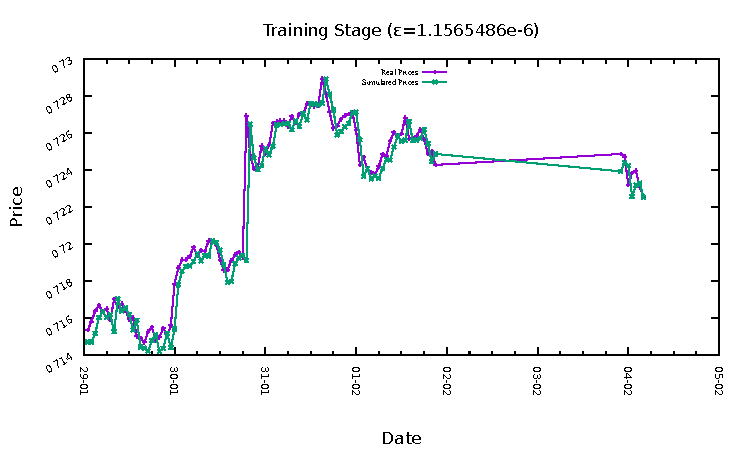
\includegraphics[width=.45\textwidth]{img/plots/aud_usd_h1-4agents-4rules-4ind-100gen_training_fit.pdf}\quad
  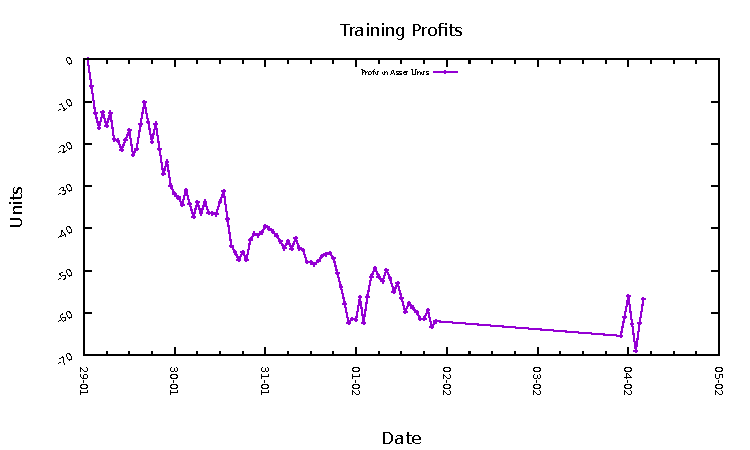
\includegraphics[width=.45\textwidth]{img/plots/aud_usd_h1-4agents-4rules-4ind-100gen_training_profits.pdf}

  \medskip

  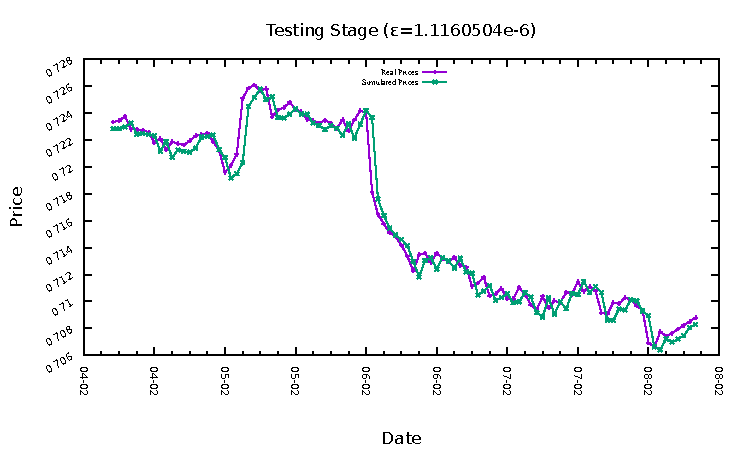
\includegraphics[width=.45\textwidth]{img/plots/aud_usd_h1-4agents-4rules-4ind-100gen_testing_fit.pdf}\quad
  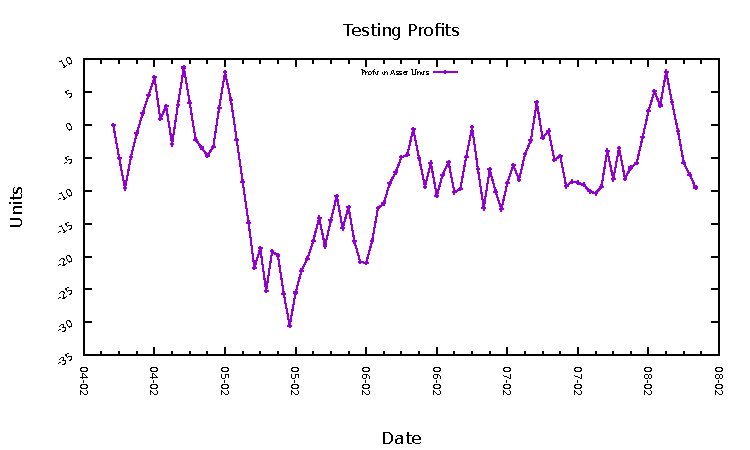
\includegraphics[width=.45\textwidth]{img/plots/aud_usd_h1-4agents-4rules-4ind-100gen_testing_profits.pdf}

  \medskip

  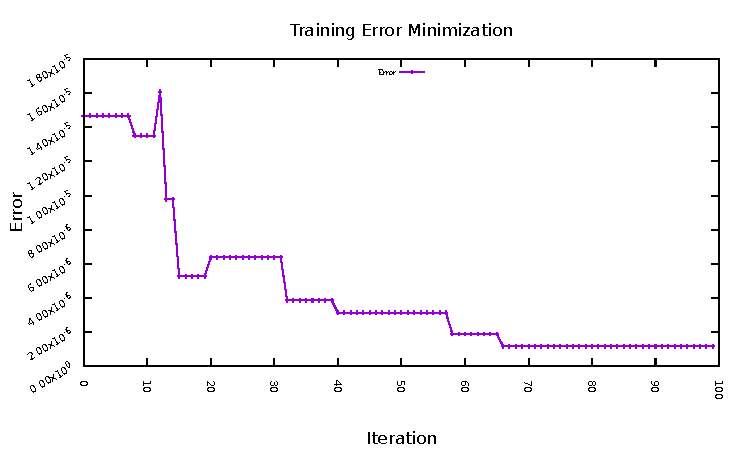
\includegraphics[width=.45\textwidth]{img/plots/aud_usd_h1-4agents-4rules-4ind-100gen_error_minimization.pdf}

  \caption{AUD/USD - 4 agents, 4 rules and 4 individuals}
  \label{figure:aud-usd-4agents-4rules-4individuals}
\end{figure}

\newpage

\subsection{AUD/USD 10 Agents, 10 Rules, 10 Individuals}
\label{results:forecast-aud-usd-10agents-10rules-10individuals}

The plots for the model generated using 10 agents with 10 rules each are shown
in Figure \ref{figure:aud-usd-10agents-10rules-10individuals}. It can be seen
that this model has better modelling capabilities than the 4 agents with 4 rules
each, as it performed better regarding profits in the training stage. However,
both models failed to obtain profits during the testing stage.

\begin{figure}[htp]
  \centering

  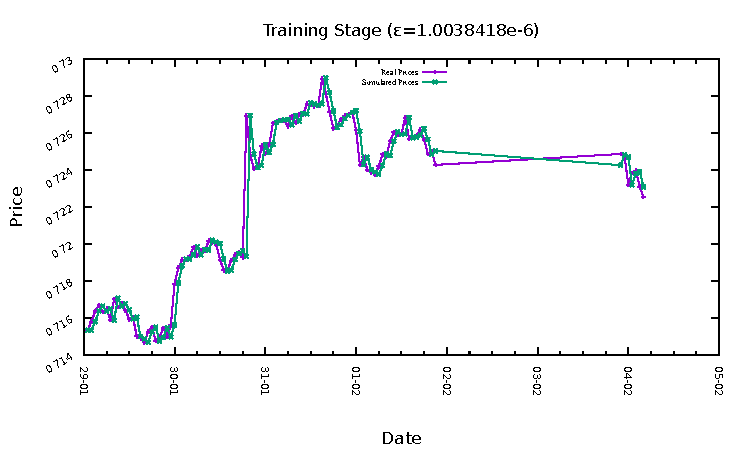
\includegraphics[width=.45\textwidth]{img/plots/aud_usd_h1-10agents-10rules-10ind-100gen_training_fit.pdf}\quad
  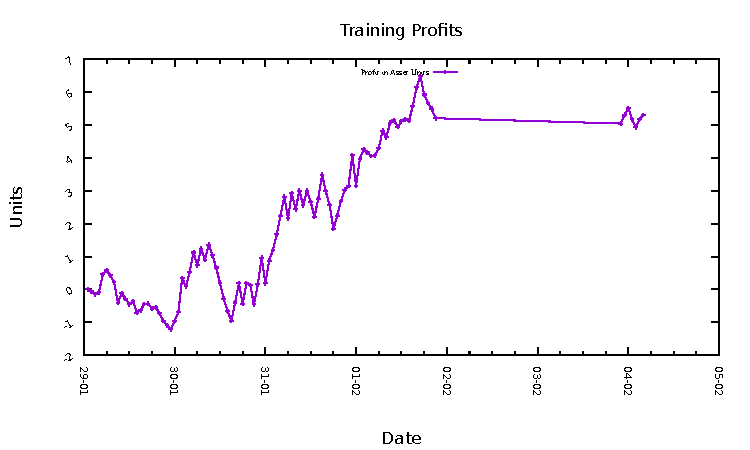
\includegraphics[width=.45\textwidth]{img/plots/aud_usd_h1-10agents-10rules-10ind-100gen_training_profits.pdf}

  \medskip

  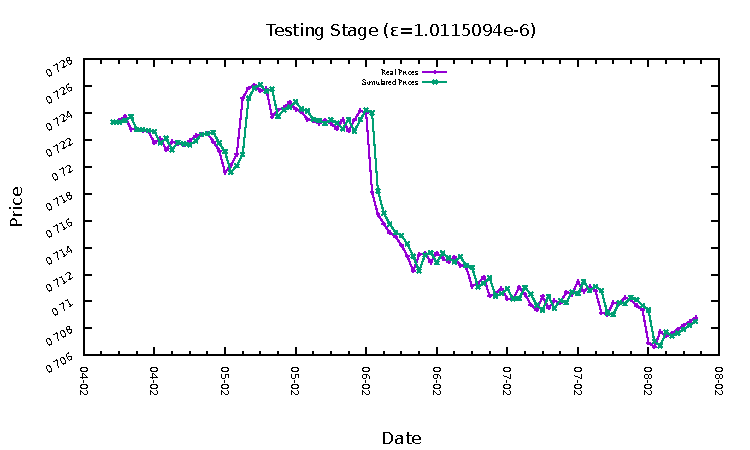
\includegraphics[width=.45\textwidth]{img/plots/aud_usd_h1-10agents-10rules-10ind-100gen_testing_fit.pdf}\quad
  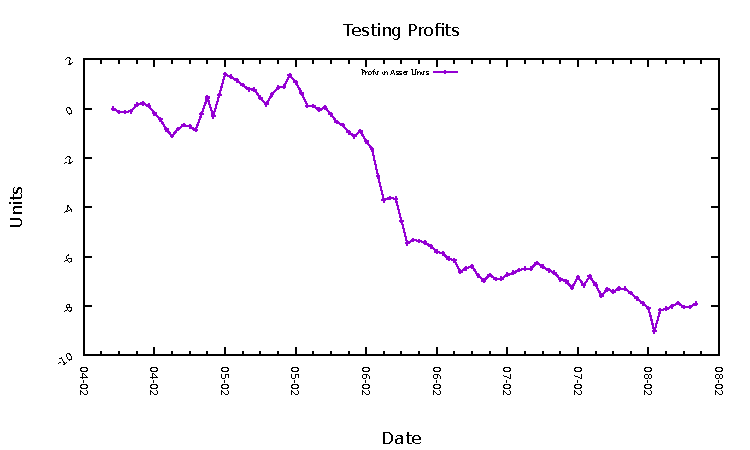
\includegraphics[width=.45\textwidth]{img/plots/aud_usd_h1-10agents-10rules-10ind-100gen_testing_profits.pdf}

  \medskip

  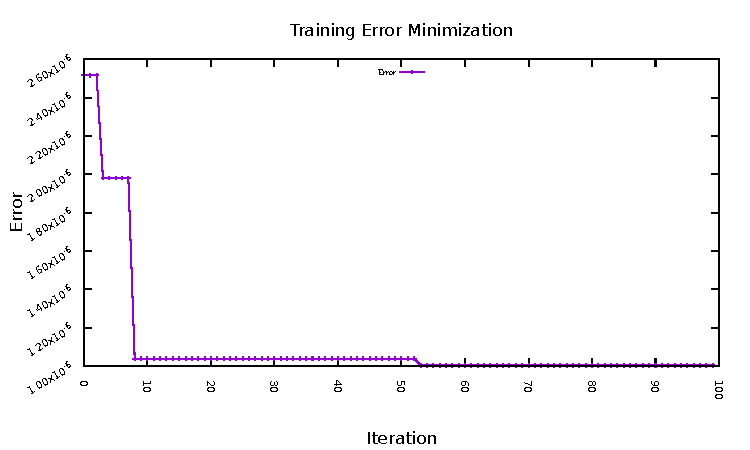
\includegraphics[width=.45\textwidth]{img/plots/aud_usd_h1-10agents-10rules-10ind-100gen_error_minimization.pdf}

  \caption{AUD/USD - 10 agents, 10 rules and 10 individuals}
  \label{figure:aud-usd-10agents-10rules-10individuals}
\end{figure}

\newpage

\subsection{AUD/USD 20 Agents, 20 Rules, 20 Individuals}
\label{results:forecast-aud-usd-20agents-20rules-20individuals}

Despite the increased modelling capabilities and diversity for the genetic
algorithm, the model generated by using 20 agents, 20 rules and 20 individuals
could not outperform the other two models for the AUD/USD. An explanation for
this is that the patterns present in the training dataset are notably different
than those found in the testing dataset, as it can be seen in Figure
\ref{figure:aud-usd-20agents-20rules-20individuals}.

\begin{figure}[htp]
  \centering

  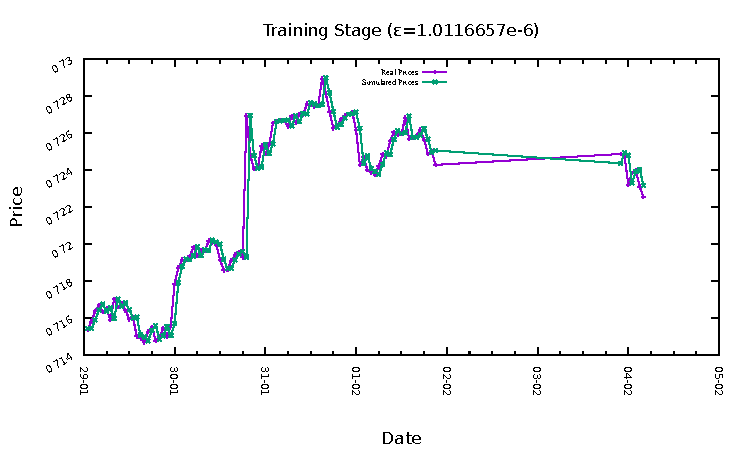
\includegraphics[width=.45\textwidth]{img/plots/aud_usd_h1-20agents-20rules-20ind-100gen_training_fit.pdf}\quad
  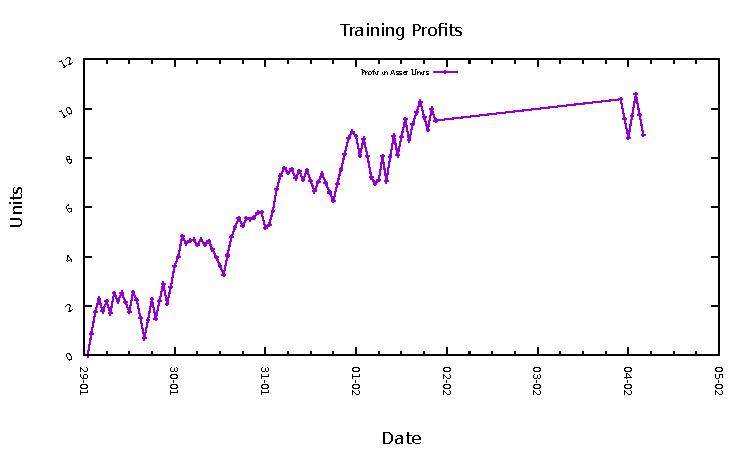
\includegraphics[width=.45\textwidth]{img/plots/aud_usd_h1-20agents-20rules-20ind-100gen_training_profits.pdf}

  \medskip

  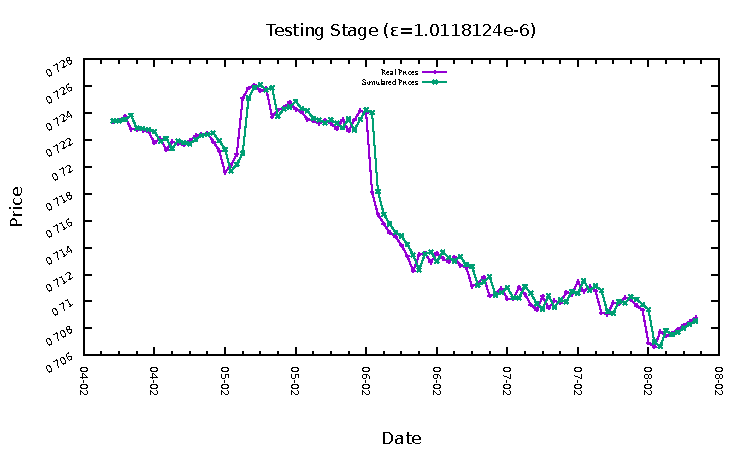
\includegraphics[width=.45\textwidth]{img/plots/aud_usd_h1-20agents-20rules-20ind-100gen_testing_fit.pdf}\quad
  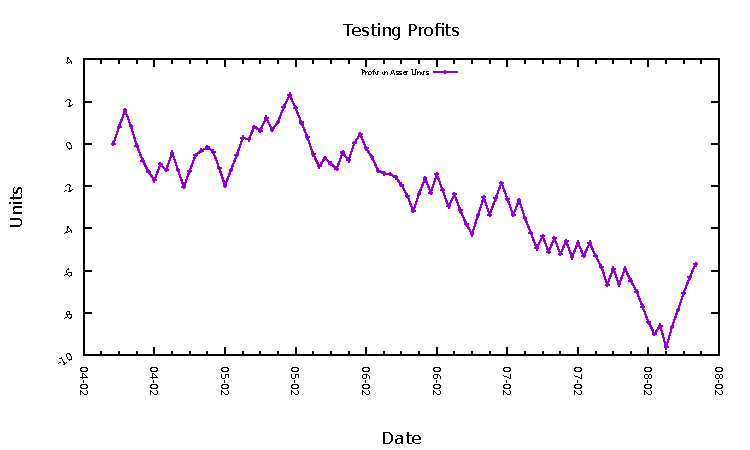
\includegraphics[width=.45\textwidth]{img/plots/aud_usd_h1-20agents-20rules-20ind-100gen_testing_profits.pdf}

  \medskip

  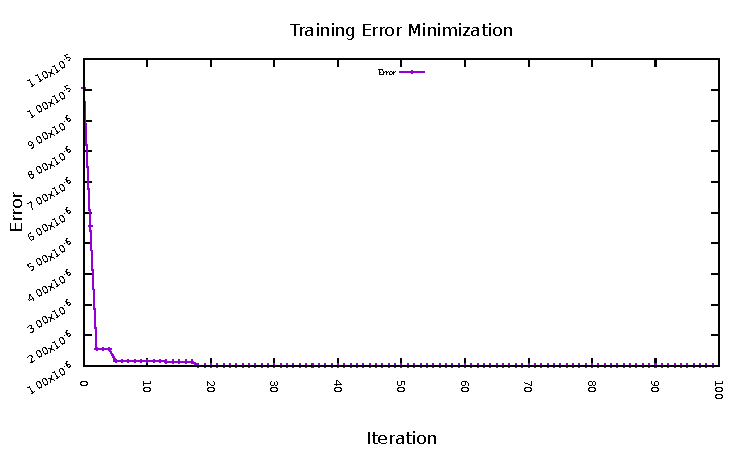
\includegraphics[width=.45\textwidth]{img/plots/aud_usd_h1-20agents-20rules-20ind-100gen_error_minimization.pdf}

  \caption{AUD/USD - 20 agents, 20 rules and 20 individuals}
  \label{figure:aud-usd-20agents-20rules-20individuals}
\end{figure}






\newpage

\subsection{EUR/GBP 4 Agents, 4 Rules, 4 Individuals}
\label{results:forecast-eur-gbp-4agents-4rules-4individuals}

Figure \ref{figure:aud-usd-20agents-20rules-20individuals} shows the plots for
the 4 agent, 4 rules, 4 individuals model. One can see that both profit plots
show bad performance. Although this is expected from this configuration, it can
also be seen that the model struggled in obtaining a simulation that resembled a
close representation of the real market, especially if it is compared to the 4
agents, 4 rules and 4 individual model for the AUD/USD market (see Figure
\ref{figure:eur-gbp-20agents-20rules-20individuals}).

\begin{figure}[htp]
  \centering

  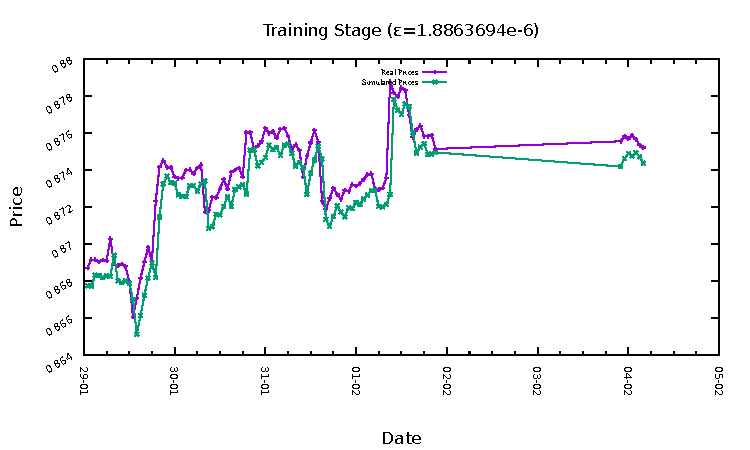
\includegraphics[width=.45\textwidth]{img/plots/eur_gbp_h1-4agents-4rules-4ind-100gen_training_fit.pdf}\quad
  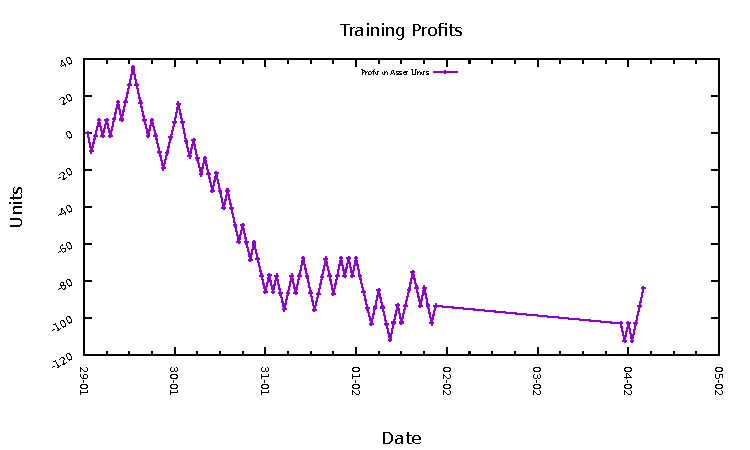
\includegraphics[width=.45\textwidth]{img/plots/eur_gbp_h1-4agents-4rules-4ind-100gen_training_profits.pdf}

  \medskip

  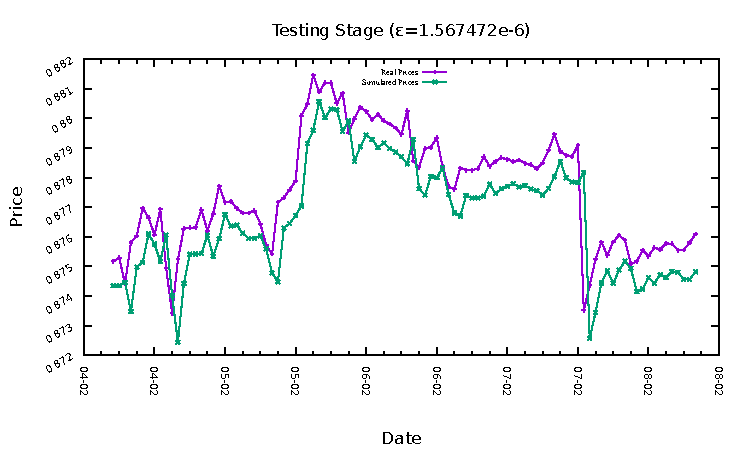
\includegraphics[width=.45\textwidth]{img/plots/eur_gbp_h1-4agents-4rules-4ind-100gen_testing_fit.pdf}\quad
  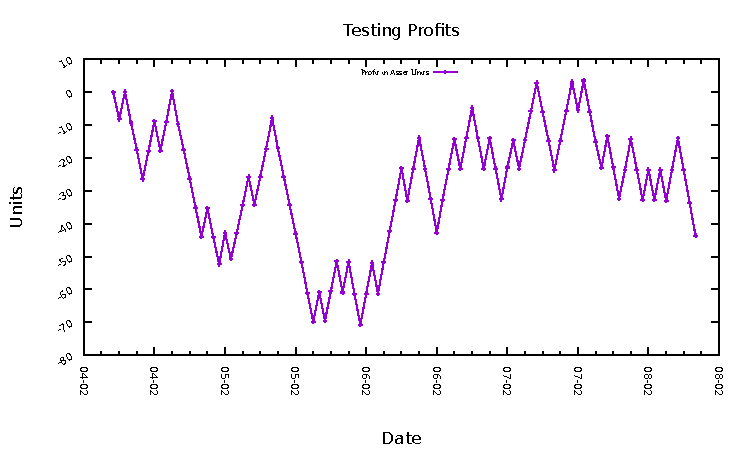
\includegraphics[width=.45\textwidth]{img/plots/eur_gbp_h1-4agents-4rules-4ind-100gen_testing_profits.pdf}

  \medskip

  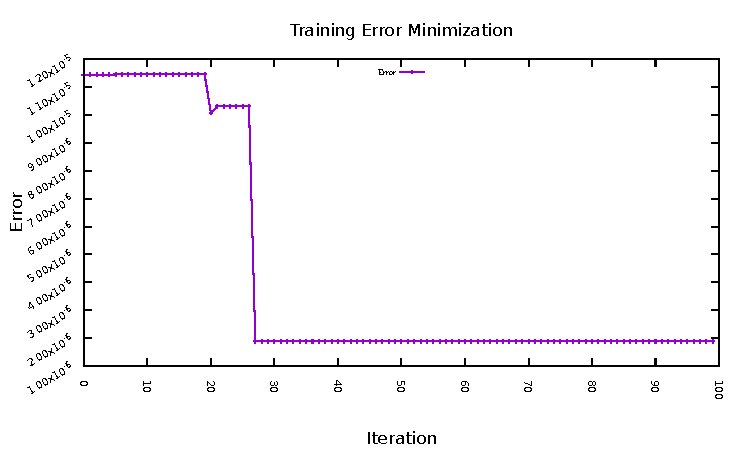
\includegraphics[width=.45\textwidth]{img/plots/eur_gbp_h1-4agents-4rules-4ind-100gen_error_minimization.pdf}

  \caption{EUR/GBP - 4 agents, 4 rules and 4 individuals}
  \label{figure:eur-gbp-4agents-4rules-4individuals}
\end{figure}

\newpage

\subsection{EUR/GBP 10 Agents, 10 Rules, 10 Individuals}
\label{results:forecast-eur-gbp-10agents-10rules-10individuals}

An interesting situation is presented in the plots in Figure
\ref{figure:eur-gbp-10agents-10rules-10individuals}. The profit plots are
identical in shape than the plots in Figure
\ref{figure:eur-gbp-4agents-4rules-4individuals}. The only inconsistency is the
magnitude of the trades, as the agents in the previous model traded more units
than the agents in this model.

\begin{figure}[htp]
  \centering

  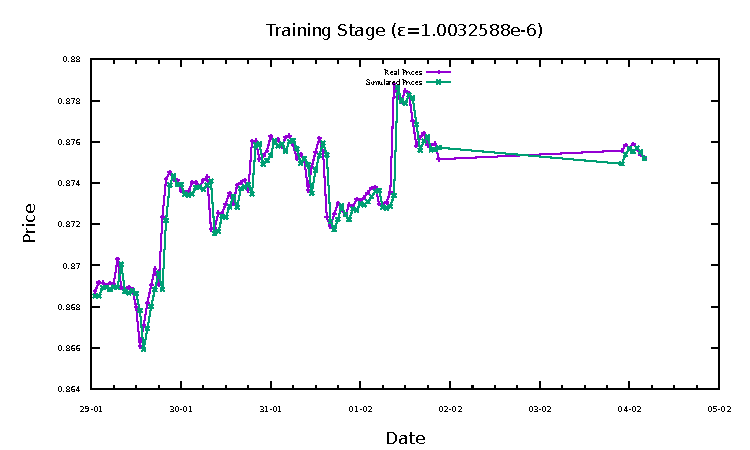
\includegraphics[width=.45\textwidth]{img/plots/eur_gbp_h1-10agents-10rules-10ind-100gen_training_fit.pdf}\quad
  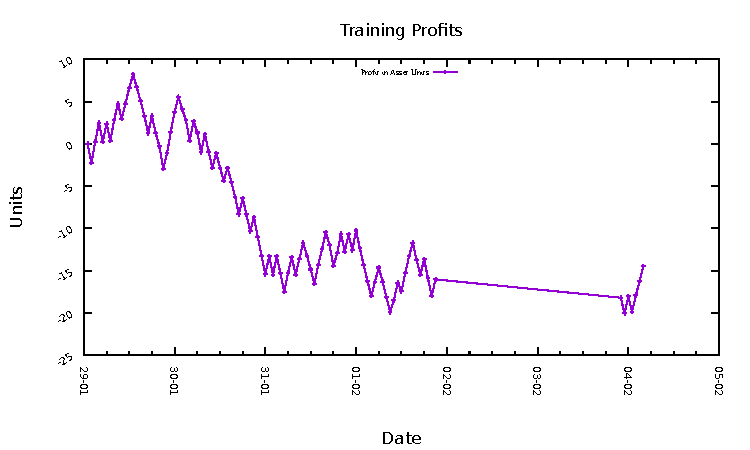
\includegraphics[width=.45\textwidth]{img/plots/eur_gbp_h1-10agents-10rules-10ind-100gen_training_profits.pdf}

  \medskip

  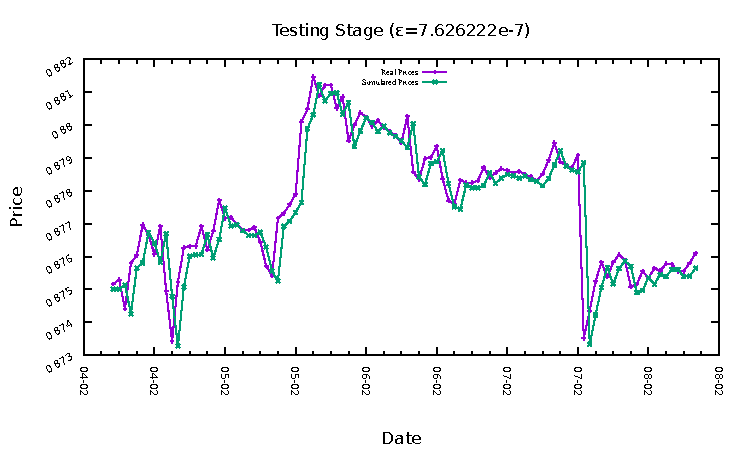
\includegraphics[width=.45\textwidth]{img/plots/eur_gbp_h1-10agents-10rules-10ind-100gen_testing_fit.pdf}\quad
  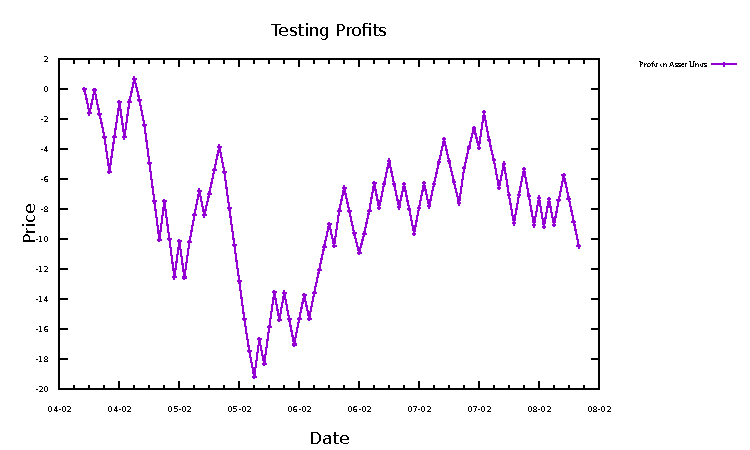
\includegraphics[width=.45\textwidth]{img/plots/eur_gbp_h1-10agents-10rules-10ind-100gen_testing_profits.pdf}

  \medskip

  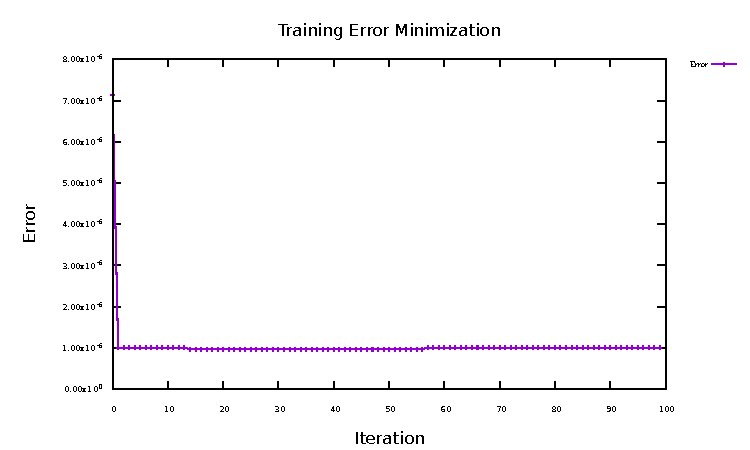
\includegraphics[width=.45\textwidth]{img/plots/eur_gbp_h1-10agents-10rules-10ind-100gen_error_minimization.pdf}

  \caption{EUR/GBP - 10 agents, 10 rules and 10 individuals}
  \label{figure:eur-gbp-10agents-10rules-10individuals}
\end{figure}

\newpage

\subsection{EUR/GBP 20 Agents, 20 Rules, 20 Individuals}
\label{results:forecast-eur-gbp-20agents-20rules-20individuals}

Although the model generated with these parameters performed well in the
training stage, as seen in Figure
\ref{figure:eur-gbp-20agents-20rules-20individuals}, it can be seen that the
model performed badly in the testing stage. However, it is worth mentioning that
the model performed well in the first 18-20 hours of the testing stage.

\begin{figure}[htp]
  \centering

  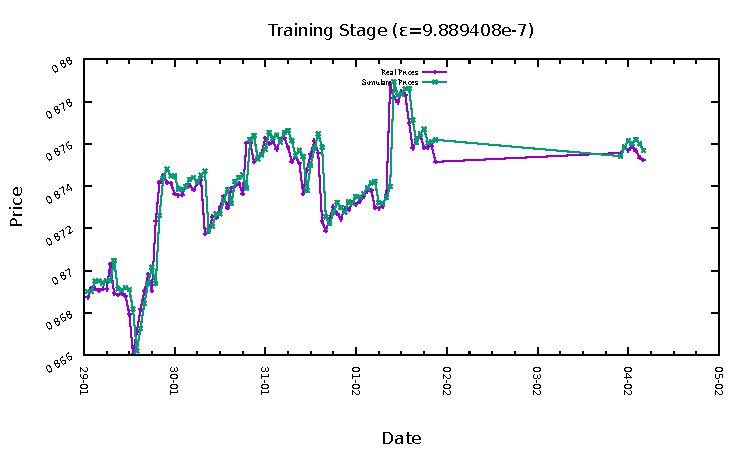
\includegraphics[width=.45\textwidth]{img/plots/eur_gbp_h1-20agents-20rules-20ind-100gen_training_fit.pdf}\quad
  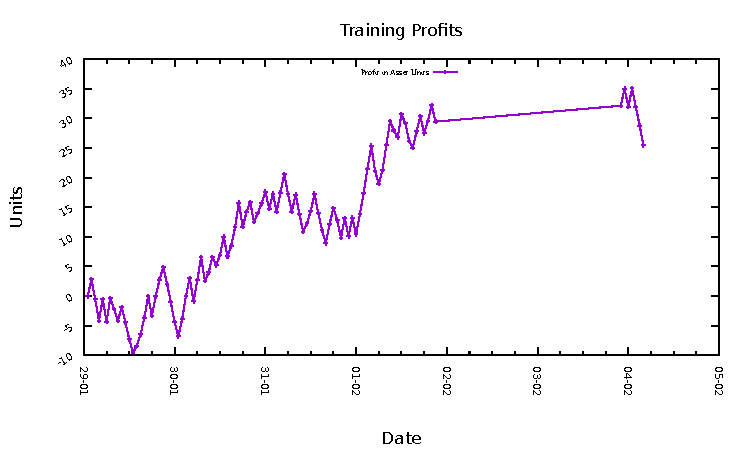
\includegraphics[width=.45\textwidth]{img/plots/eur_gbp_h1-20agents-20rules-20ind-100gen_training_profits.pdf}

  \medskip

  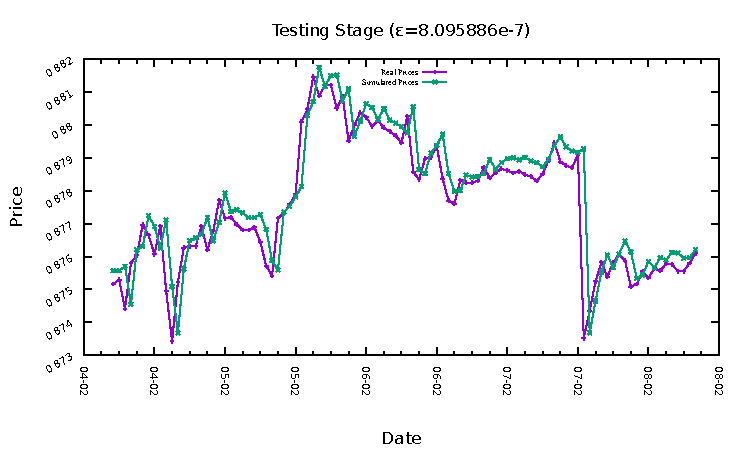
\includegraphics[width=.45\textwidth]{img/plots/eur_gbp_h1-20agents-20rules-20ind-100gen_testing_fit.pdf}\quad
  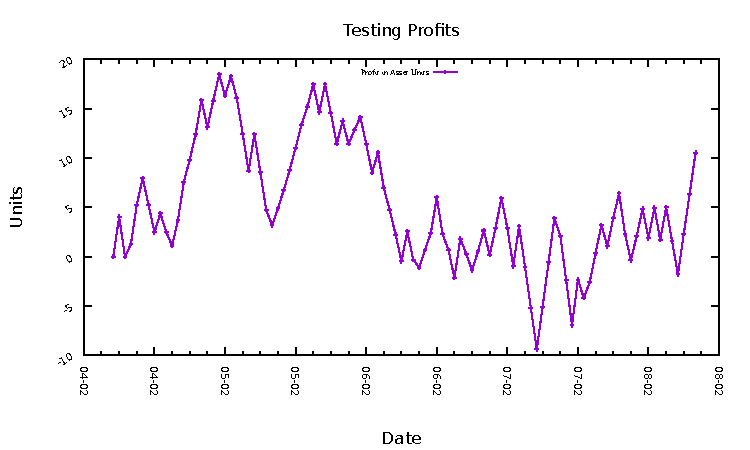
\includegraphics[width=.45\textwidth]{img/plots/eur_gbp_h1-20agents-20rules-20ind-100gen_testing_profits.pdf}

  \medskip

  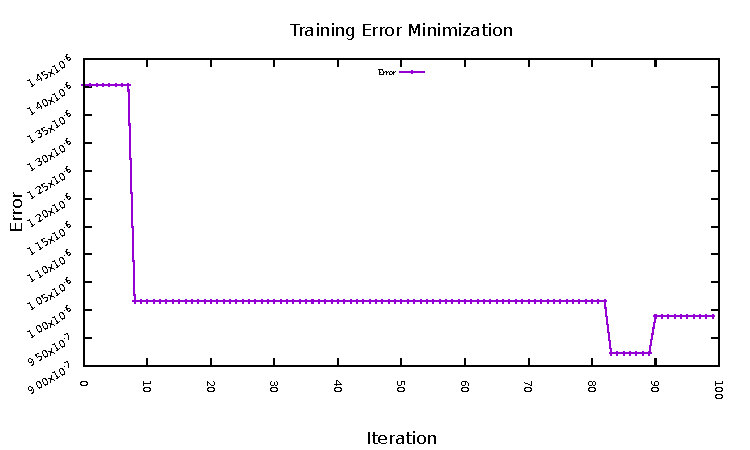
\includegraphics[width=.45\textwidth]{img/plots/eur_gbp_h1-20agents-20rules-20ind-100gen_error_minimization.pdf}

  \caption{EUR/GBP - 20 agents, 20 rules and 20 individuals}
  \label{figure:eur-gbp-20agents-20rules-20individuals}
\end{figure}




\newpage

\subsection{EUR/USD 4 Agents, 4 Rules, 4 Individuals}
\label{results:forecast-eur-usd-4agents-4rules-4individuals}

This model can be seen how badly it performed in the testing stage, as shown in
Figure \ref{figure:eur-usd-4agents-4rules-4individuals}. However, it performed
well in the training stage. It must also be noted that a bad performance can be
expected due to the differences in the patterns between the training and testing
datasets.

\begin{figure}[htp]
  \centering

  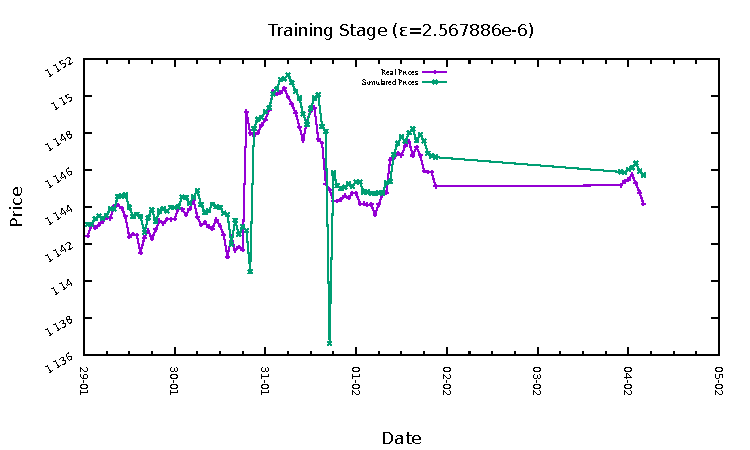
\includegraphics[width=.45\textwidth]{img/plots/eur_usd_h1-4agents-4rules-4ind-100gen_training_fit.pdf}\quad
  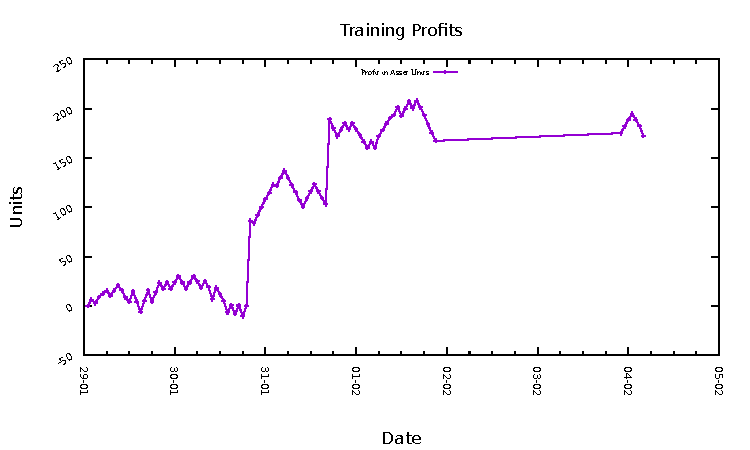
\includegraphics[width=.45\textwidth]{img/plots/eur_usd_h1-4agents-4rules-4ind-100gen_training_profits.pdf}

  \medskip

  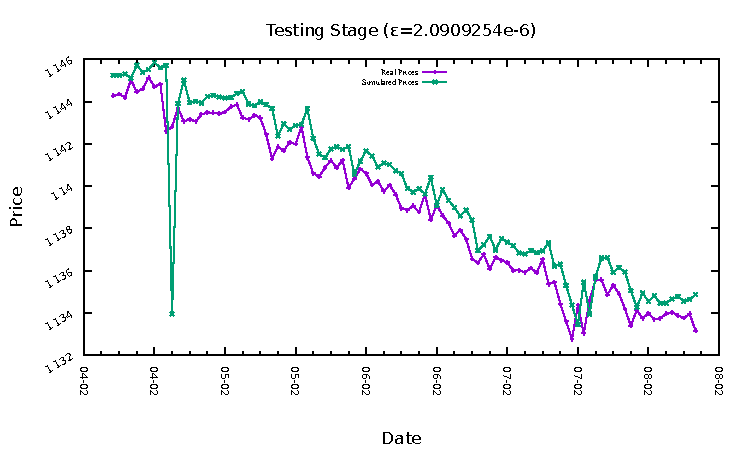
\includegraphics[width=.45\textwidth]{img/plots/eur_usd_h1-4agents-4rules-4ind-100gen_testing_fit.pdf}\quad
  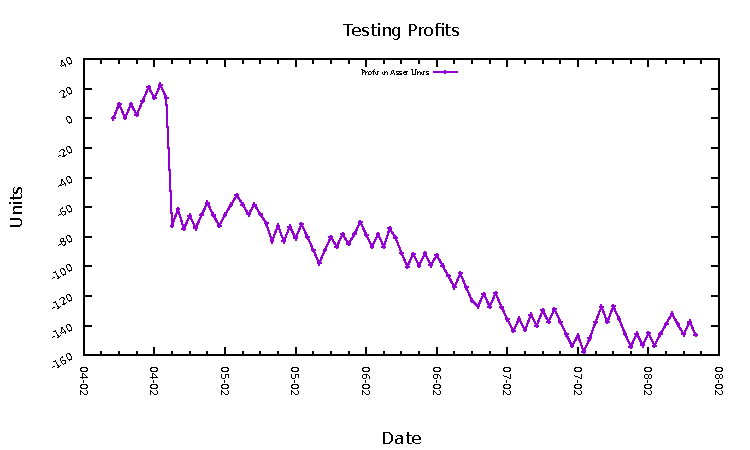
\includegraphics[width=.45\textwidth]{img/plots/eur_usd_h1-4agents-4rules-4ind-100gen_testing_profits.pdf}

  \medskip

  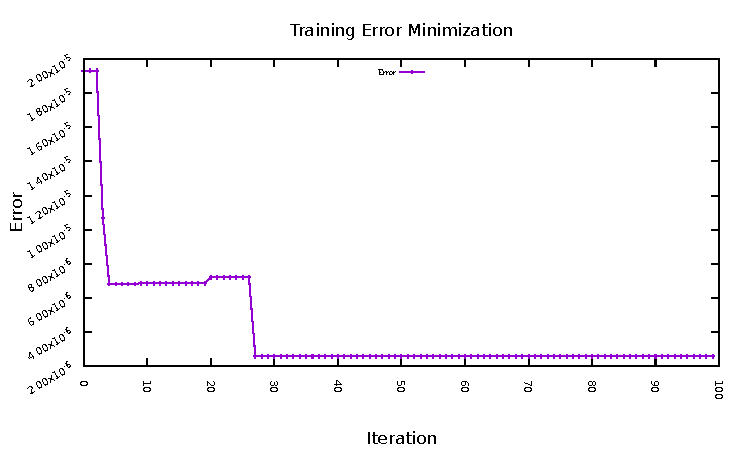
\includegraphics[width=.45\textwidth]{img/plots/eur_usd_h1-4agents-4rules-4ind-100gen_error_minimization.pdf}

  \caption{EUR/USD - 4 agents, 4 rules and 4 individuals}
  \label{figure:eur-usd-4agents-4rules-4individuals}
\end{figure}

\newpage

\subsection{EUR/USD 10 Agents, 10 Rules, 10 Individuals}
\label{results:forecast-eur-usd-10agents-10rules-10individuals}

The plots in Figure \ref{figure:eur-usd-10agents-10rules-10individuals}
demonstrate an improvement regarding the curve-fitting capabilities of the model
compared to the previous model for the EUR/USD market. This is surprising, given
the differences in patterns between the two datasets. Additionally, it can be
noted that the model performed well in both the training and testing stages,
despite the model performing badly in the last hours of the testing stage.

\begin{figure}[htp]
  \centering

  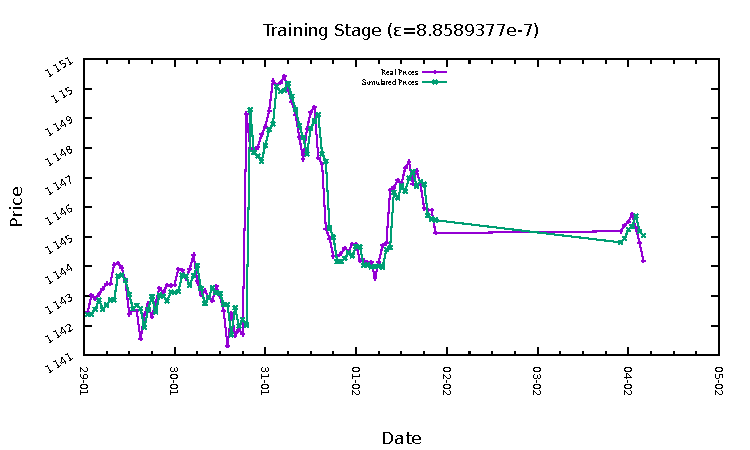
\includegraphics[width=.45\textwidth]{img/plots/eur_usd_h1-10agents-10rules-10ind-100gen_training_fit.pdf}\quad
  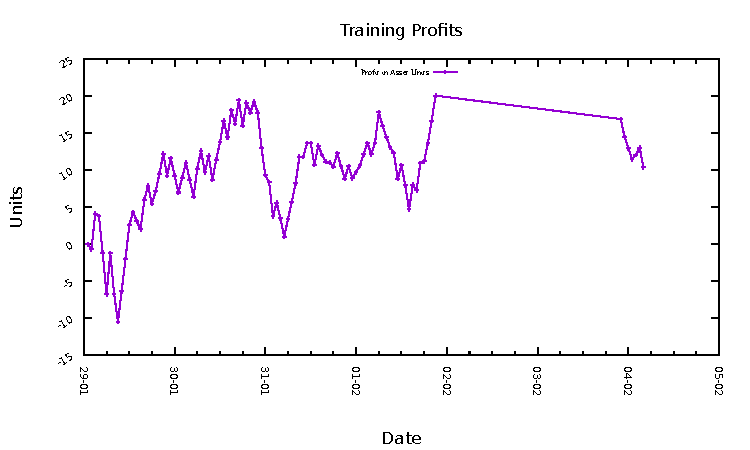
\includegraphics[width=.45\textwidth]{img/plots/eur_usd_h1-10agents-10rules-10ind-100gen_training_profits.pdf}

  \medskip

  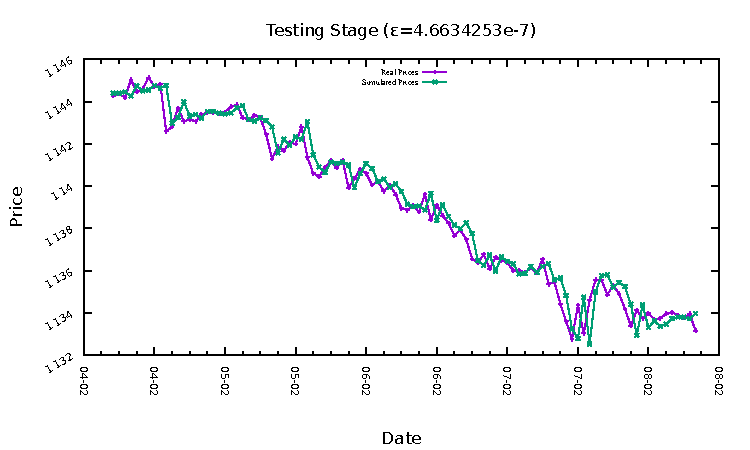
\includegraphics[width=.45\textwidth]{img/plots/eur_usd_h1-10agents-10rules-10ind-100gen_testing_fit.pdf}\quad
  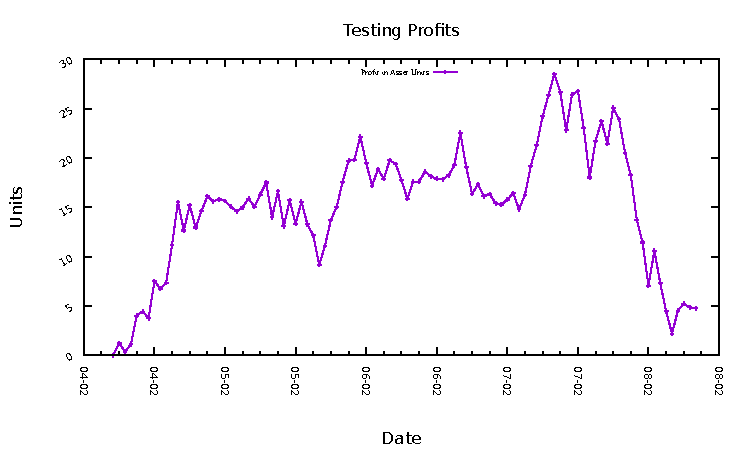
\includegraphics[width=.45\textwidth]{img/plots/eur_usd_h1-10agents-10rules-10ind-100gen_testing_profits.pdf}

  \medskip

  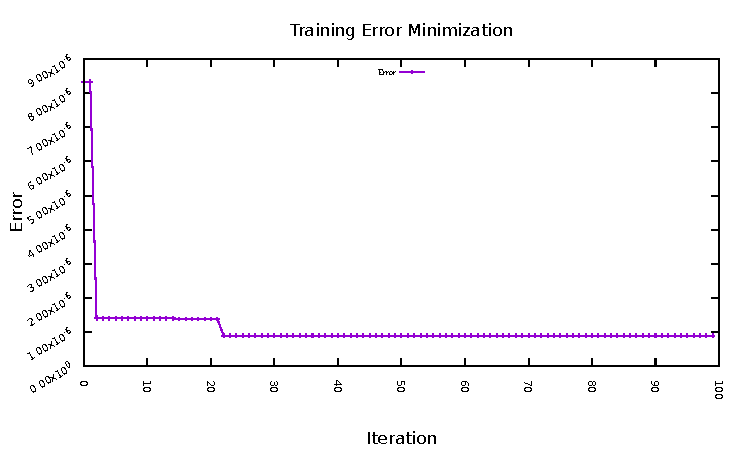
\includegraphics[width=.45\textwidth]{img/plots/eur_usd_h1-10agents-10rules-10ind-100gen_error_minimization.pdf}

  \caption{EUR/USD - 10 agents, 10 rules and 10 individuals}
  \label{figure:eur-usd-10agents-10rules-10individuals}
\end{figure}

\newpage

\subsection{EUR/USD 20 Agents, 20 Rules, 20 Individuals}
\label{results:forecast-eur-usd-20agents-20rules-20individuals}

The model represented by the plots in Figure
\ref{figure:eur-usd-20agents-20rules-20individuals} is seen to have performed
badly in both the training and testing stages. A possible explanation for this
behavior is that more generations would be required in order for the model to
extract a generalization of the market, as a consequence of the high number of
agents and rules.

\begin{figure}[htp]
  \centering

  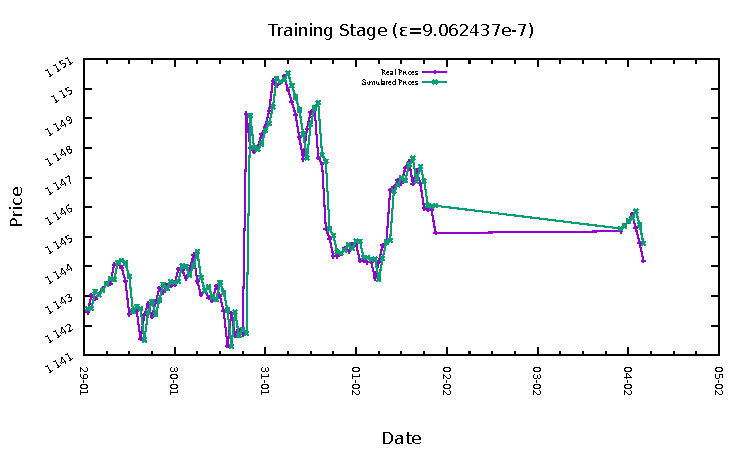
\includegraphics[width=.45\textwidth]{img/plots/eur_usd_h1-20agents-20rules-20ind-100gen_training_fit.pdf}\quad
  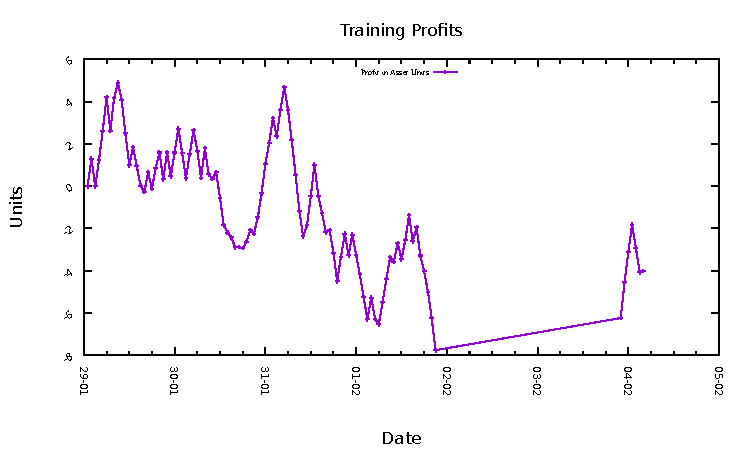
\includegraphics[width=.45\textwidth]{img/plots/eur_usd_h1-20agents-20rules-20ind-100gen_training_profits.pdf}

  \medskip

  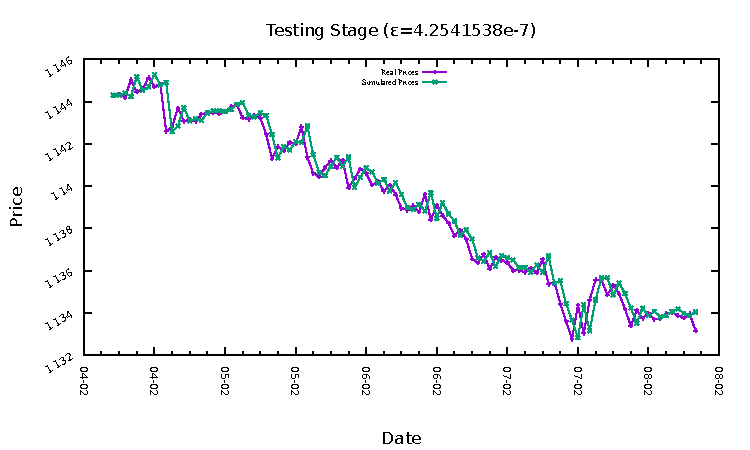
\includegraphics[width=.45\textwidth]{img/plots/eur_usd_h1-20agents-20rules-20ind-100gen_testing_fit.pdf}\quad
  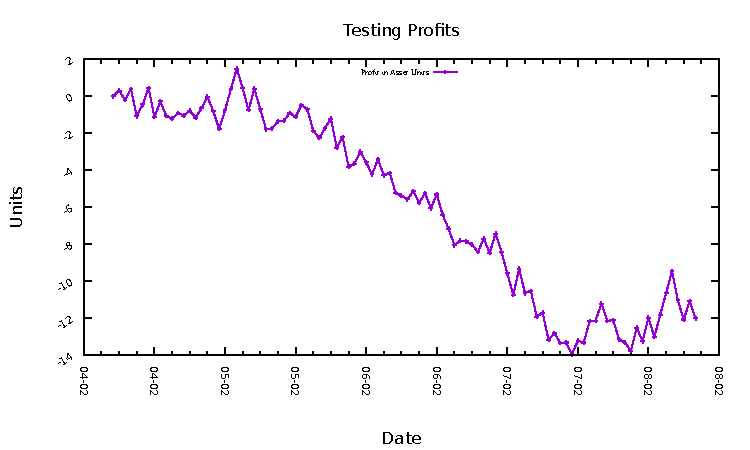
\includegraphics[width=.45\textwidth]{img/plots/eur_usd_h1-20agents-20rules-20ind-100gen_testing_profits.pdf}

  \medskip

  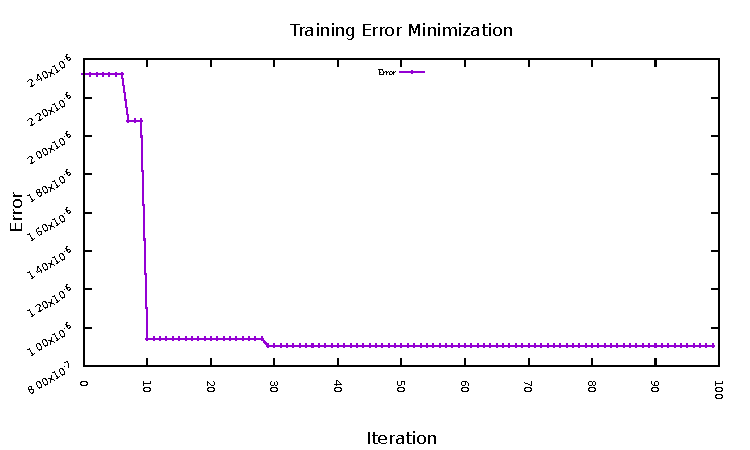
\includegraphics[width=.45\textwidth]{img/plots/eur_usd_h1-20agents-20rules-20ind-100gen_error_minimization.pdf}

  \caption{EUR/USD - 20 agents, 20 rules and 20 individuals}
  \label{figure:eur-usd-20agents-20rules-20individuals}
\end{figure}




\newpage

\subsection{GBP/USD 4 Agents, 4 Rules, 4 Individuals}
\label{results:forecast-gbp-usd-4agents-4rules-4individuals}

As expected from a model with poor modelling capabilities, the profit plots in
Figure \ref{figure:gbp-usd-4agents-4rules-4individuals} show that the model was
not able to simulate the patterns of the GBP/USD market.

\begin{figure}[htp]
  \centering

  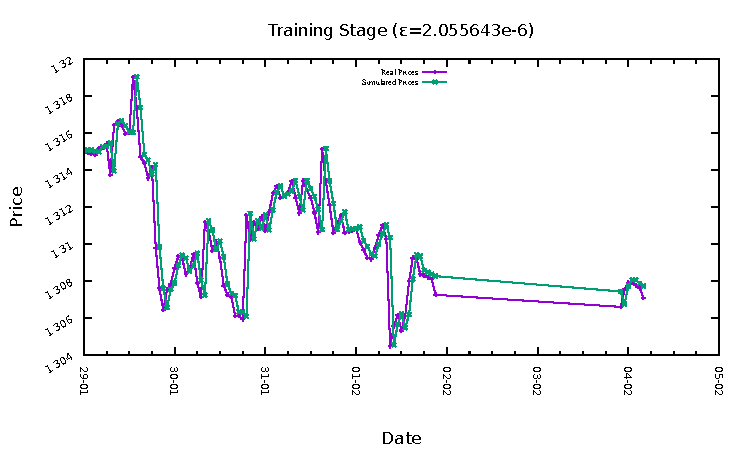
\includegraphics[width=.45\textwidth]{img/plots/gbp_usd_h1-4agents-4rules-4ind-100gen_training_fit.pdf}\quad
  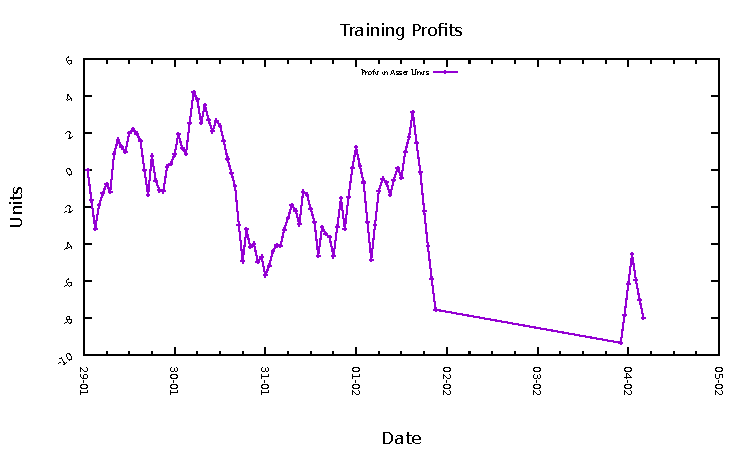
\includegraphics[width=.45\textwidth]{img/plots/gbp_usd_h1-4agents-4rules-4ind-100gen_training_profits.pdf}

  \medskip

  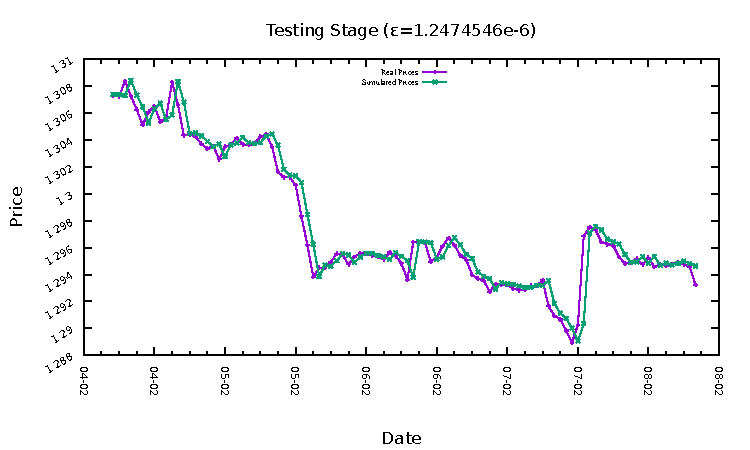
\includegraphics[width=.45\textwidth]{img/plots/gbp_usd_h1-4agents-4rules-4ind-100gen_testing_fit.pdf}\quad
  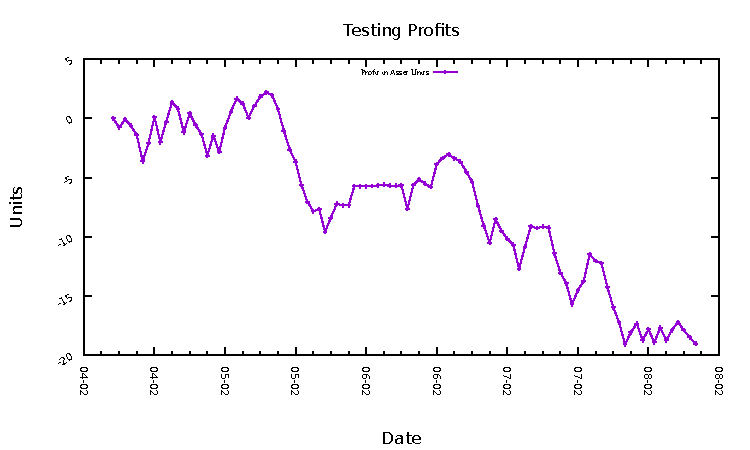
\includegraphics[width=.45\textwidth]{img/plots/gbp_usd_h1-4agents-4rules-4ind-100gen_testing_profits.pdf}

  \medskip

  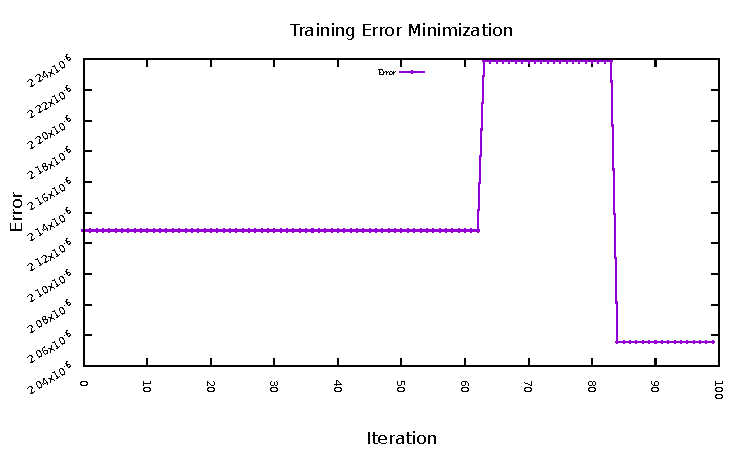
\includegraphics[width=.45\textwidth]{img/plots/gbp_usd_h1-4agents-4rules-4ind-100gen_error_minimization.pdf}

  \caption{GBP/USD - 4 agents, 4 rules and 4 individuals}
  \label{figure:gbp-usd-4agents-4rules-4individuals}
\end{figure}

\newpage

\subsection{GBP/USD 10 Agents, 10 Rules, 10 Individuals}
\label{results:forecast-gbp-usd-10agents-10rules-10individuals}

In the case of this model for the GBP/USD market, a remarkable performance can
be noticed in Figure \ref{figure:gbp-usd-10agents-10rules-10individuals} in the
profit plots for both the training and testing stages.

\begin{figure}[htp]
  \centering

  \includegraphics[width=.45\textwidth]{img/plots/gbp_usd_h1-10agents-10rules-10ind-100gen_training_fit.pdf}\quad
  \includegraphics[width=.45\textwidth]{img/plots/gbp_usd_h1-10agents-10rules-10ind-100gen_training_profits.pdf}

  \medskip

  \includegraphics[width=.45\textwidth]{img/plots/gbp_usd_h1-10agents-10rules-10ind-100gen_testing_fit.pdf}\quad
  \includegraphics[width=.45\textwidth]{img/plots/gbp_usd_h1-10agents-10rules-10ind-100gen_testing_profits.pdf}

  \medskip

  \includegraphics[width=.45\textwidth]{img/plots/gbp_usd_h1-10agents-10rules-10ind-100gen_error_minimization.pdf}

  \caption{GBP/USD - 10 agents, 10 rules and 10 individuals}
  \label{figure:gbp-usd-10agents-10rules-10individuals}
\end{figure}

\newpage

\subsection{GBP/USD 20 Agents, 20 Rules, 20 Individuals}
\label{results:forecast-gbp-usd-20agents-20rules-20individuals}

In contrast to other models using 20 agents with 20 rules each, the model
represented by the plots in Figure
\ref{figure:gbp-usd-20agents-20rules-20individuals} is shown to perform well in
both the training and testing stages regarding the accumulated profits, although
the profits do not reach a similar magnitude as the previous model.

\begin{figure}[htp]
  \centering

  \includegraphics[width=.45\textwidth]{img/plots/gbp_usd_h1-20agents-20rules-20ind-100gen_training_fit.pdf}\quad
  \includegraphics[width=.45\textwidth]{img/plots/gbp_usd_h1-20agents-20rules-20ind-100gen_training_profits.pdf}

  \medskip

  \includegraphics[width=.45\textwidth]{img/plots/gbp_usd_h1-20agents-20rules-20ind-100gen_testing_fit.pdf}\quad
  \includegraphics[width=.45\textwidth]{img/plots/gbp_usd_h1-20agents-20rules-20ind-100gen_testing_profits.pdf}

  \medskip

  \includegraphics[width=.45\textwidth]{img/plots/gbp_usd_h1-20agents-20rules-20ind-100gen_error_minimization.pdf}

  \caption{GBP/USD - 20 agents, 20 rules and 20 individuals}
  \label{figure:gbp-usd-20agents-20rules-20individuals}
\end{figure}







\newpage

\subsection{USD/CAD 4 Agents, 4 Rules, 4 Individuals}
\label{results:forecast-usd-cad-4agents-4rules-4individuals}

The plots in Figure \ref{figure:usd-cad-4agents-4rules-4individuals} present an
interesting situation: the model seems to perform badly regarding profits in the
training stage, but not in the testing stage. This behavior is clearer after
examining the plots of the training and testing datasets: one exhibits a
downtrend market direction, while the other shiftes to a clear uptrend. The
model learned how to perform badly in a downtrend market, but it performed well
in the testing stage because of the shift in direction.

\begin{figure}[htp]
  \centering

  \includegraphics[width=.45\textwidth]{img/plots/usd_cad_h1-4agents-4rules-4ind-100gen_training_fit.pdf}\quad
  \includegraphics[width=.45\textwidth]{img/plots/usd_cad_h1-4agents-4rules-4ind-100gen_training_profits.pdf}

  \medskip

  \includegraphics[width=.45\textwidth]{img/plots/usd_cad_h1-4agents-4rules-4ind-100gen_testing_fit.pdf}\quad
  \includegraphics[width=.45\textwidth]{img/plots/usd_cad_h1-4agents-4rules-4ind-100gen_testing_profits.pdf}

  \medskip

  \includegraphics[width=.45\textwidth]{img/plots/usd_cad_h1-4agents-4rules-4ind-100gen_error_minimization.pdf}

  \caption{USD/CAD - 4 agents, 4 rules and 4 individuals}
  \label{figure:usd-cad-4agents-4rules-4individuals}
\end{figure}

\newpage

\subsection{USD/CAD 10 Agents, 10 Rules, 10 Individuals}
\label{results:forecast-usd-cad-10agents-10rules-10individuals}

In contrast to the previous model, the model represented by the plots shown in
Figure \ref{figure:usd-cad-10agents-10rules-10individuals} performs badly in the
testing stage, most likely because of the nature of the training dataset which
sharply contrasts with the nature of the testing dataset.

\begin{figure}[htp]
  \centering

  \includegraphics[width=.45\textwidth]{img/plots/usd_cad_h1-10agents-10rules-10ind-100gen_training_fit.pdf}\quad
  \includegraphics[width=.45\textwidth]{img/plots/usd_cad_h1-10agents-10rules-10ind-100gen_training_profits.pdf}

  \medskip

  \includegraphics[width=.45\textwidth]{img/plots/usd_cad_h1-10agents-10rules-10ind-100gen_testing_fit.pdf}\quad
  \includegraphics[width=.45\textwidth]{img/plots/usd_cad_h1-10agents-10rules-10ind-100gen_testing_profits.pdf}

  \medskip

  \includegraphics[width=.45\textwidth]{img/plots/usd_cad_h1-10agents-10rules-10ind-100gen_error_minimization.pdf}

  \caption{USD/CAD - 10 agents, 10 rules and 10 individuals}
  \label{figure:usd-cad-10agents-10rules-10individuals}
\end{figure}

\newpage

\subsection{USD/CAD 20 Agents, 20 Rules, 20 Individuals}
\label{results:forecast-usd-cad-20agents-20rules-20individuals}

The model represented by the plots in Figure
\ref{figure:usd-cad-20agents-20rules-20individuals} performs similarly to the
previously discussed model. The explanation behind this behavior should be the
same as the one mentioned in the previous Subsection.

\begin{figure}[htp]
  \centering

  \includegraphics[width=.45\textwidth]{img/plots/usd_cad_h1-20agents-20rules-20ind-100gen_training_fit.pdf}\quad
  \includegraphics[width=.45\textwidth]{img/plots/usd_cad_h1-20agents-20rules-20ind-100gen_training_profits.pdf}

  \medskip

  \includegraphics[width=.45\textwidth]{img/plots/usd_cad_h1-20agents-20rules-20ind-100gen_testing_fit.pdf}\quad
  \includegraphics[width=.45\textwidth]{img/plots/usd_cad_h1-20agents-20rules-20ind-100gen_testing_profits.pdf}

  \medskip

  \includegraphics[width=.45\textwidth]{img/plots/usd_cad_h1-20agents-20rules-20ind-100gen_error_minimization.pdf}

  \caption{USD/CAD - 20 agents, 20 rules and 20 individuals}
  \label{figure:usd-cad-20agents-20rules-20individuals}
\end{figure}



\newpage

\section{Extracting Insights about a Financial Market}
\label{section:extracting-insights-about-a-financial-market}

This Section shows interpretations of two different foreign exchange markets
obtained by examining the agents in the agent-based models generated for the
experiments shown in Section
\ref{section:forecasting-the-prices-of-a-financial-market}. Only the two markets
are presented in this Section as they are enough to demonstrate their use. The
rest of the interpretetations for the markets described in Section
\ref{section:forecasting-the-prices-of-a-financial-market} can be found in
Appendix \ref{app:market-interpretations}, and the full list of interpretations
for all the experiments performed can be found in the git repository of this
thesis document. The interpretations
consist of a series of sentences, where each give a summary of the profits,
perceptions, hesitancy and actions of groups of agents. Considering the
following sentence: ``3 agents — with an average profit of 68 units — perceived
in 85\% of the market that a weak resistance above current price — with a
hesitancy of 0.147 — is a signal to sell — with a hesitancy of 0.079.'', one can
draw the following conclusions about 3 agents in a community of agents: their
average profit in a dataset is of 68 units; in 85\% of the data points in the
dataset, they perceived that a price area with a low weight above the current
price is a signal to sell; after perceiving a low weight price area, they add
some hesitancy or doubt to their perception, and then they decide to sell, but
this decision has also some hesitancy or doubt. Hesitancy or doubt (see Section
\ref{section:using-the-agent-based-model-to-generate-insights-about-a-financial-market})
in this case is an indicative of how significant the perception has to be in
order to be indeed perceived as a low weight price area, and how many units are
actually traded; it can be seen as penalties to the agent's perception and
action.

The following interpretations show five sentences for the training stage of the
model and five sentences for the testing stage. These only represent excerpts of
the generated interpretations; it was decided for them to be truncated due to
space constraints in this thesis document, but the reader can find the full
interpretations in this thesis' Git repository. In order to obtain these five
sentence excerpts, all the generated sentences were ordered by the number of
agents and then by the number of units in profits. This way the sentences show
where the most number of agents in the community of agents coincided in their
perceptions and decisions, and then show what situations were the more
profitable.

%% Interpretations for the five foreign exchange markets AUD/USD, EUR/GBP, EUR/USD,
%% GBP/USD and USD/CAD are included. Each of these markets show interpretations for
%% the models with the following variants in parameters: 4 agents, 4 rules and 4
%% individuals; 10 agents, 10 rules and 10 individuals; 20 agents, 20 rules and 20
%% individuals.

\subsection{AUD/USD 4 Agents, 4 Rules, 4 Individuals}

One can see in the first sentence of the training set that 3 agents decided to
trade when a weak resistance is presented above the current price. In the
training stage these agents were not profitable, while in the testing stage they
were profitable. This indicates that this pattern is not as reliable as, for
example, the one presented in the second sentence in the training set, where
agents decided to buy when they perceived a weak resistance nearby the current
price. This behavior showed to also be profitable in the testing stage, as is
shown in the fourth sentence of the corresponding set.

\subsubsection{Training}

{\small
  \begin{itemize}
  \item 3 agents — with an average profit of -68 units — perceived in 68\% of
    the market that a weak resistance above current price — with a hesitancy of
    0.147 — is a signal to sell — with a hesitancy of 0.079.
  \item 2 agents — with an average profit of 280 units — perceived in 46\% of
    the market that a weak resistance nearby current price — with a hesitancy of
    0.133 — is a signal to buy — with a hesitancy of 0.097.
  \item 2 agents — with an average profit of 280 units — perceived in 22\% of
    the market that a moderate resistance above current price — with a hesitancy
    of 0.15 — is a signal to buy — with a hesitancy of 0.113.
  \item 2 agents — with an average profit of 38 units — perceived in 56\% of the
    market that a weak resistance below current price — with a hesitancy of
    0.246 — is a signal to buy — with a hesitancy of 0.094.
  \item 2 agents — with an average profit of -41 units — perceived in 56\% of
    the market that a weak resistance below current price — with a hesitancy of
    0.009 — is a signal to sell — with a hesitancy of 0.132.
  \end{itemize}
}

\subsubsection{Testing}

{\small
  \begin{itemize}
  \item 3 agents — with an average profit of 68 units — perceived in 85\% of the
    market that a weak resistance above current price — with a hesitancy of
    0.147 — is a signal to sell — with a hesitancy of 0.079.
  \item 2 agents — with an average profit of 352 units — perceived in 47\% of
    the market that a moderate resistance below current price — with a hesitancy
    of 0.134 — is a signal to sell — with a hesitancy of 0.151.
  \item 2 agents — with an average profit of 323 units — perceived in 6\% of the
    market that a strong resistance below current price — with a hesitancy of
    0.098 — is a signal to sell — with a hesitancy of 0.024.
  \item 2 agents — with an average profit of 323 units — perceived in 55\% of
    the market that a weak resistance nearby current price — with a hesitancy of
    0.04 — is a signal to sell — with a hesitancy of 0.138.
  \item 2 agents — with an average profit of 309 units — perceived in 0\% of the
    market that a strong resistance above current price — with a hesitancy of
    0.127 — is a signal to sell — with a hesitancy of 0.14.
  \end{itemize}
}

\subsection{EUR/GBP 4 Agents, 4 Rules, 4 Individuals}

An interesting situation in these sets of interpretations is that the only
sentence in the training set that signals an actual trade action is among the
most profitable interpretations in the testing stage -- but with a 0\% of
perception in the market. This can also be seen as a signal to not follow the
behavior presented by this model, which agrees the profit plots of the model
presented in the previous Section.

\subsubsection{Training}

{\small
  \begin{itemize}
  \item 3 agents — with an average profit of 60 units — perceived in 56\% of the
    market that a weak resistance above current price — with a hesitancy of
    0.094 — is a signal to hold the current position — with a hesitancy of
    0.029.
  \item 3 agents — with an average profit of 31 units — perceived in 36\% of the
    market that a moderate resistance nearby current price — with a hesitancy of
    0.126 — is a signal to hold the current position — with a hesitancy of
    0.194.
  \item 3 agents — with an average profit of -44 units — perceived in 13\% of
    the market that a strong resistance below current price — with a hesitancy
    of 0.044 — is a signal to hold the current position — with a hesitancy of
    0.152.
  \item 2 agents — with an average profit of 105 units — perceived in 13\% of
    the market that a strong resistance below current price — with a hesitancy
    of 0.114 — is a signal to sell — with a hesitancy of 0.102.
  \item 2 agents — with an average profit of 105 units — perceived in 42\% of
    the market that a weak resistance nearby current price — with a hesitancy of
    0.105 — is a signal to hold the current position — with a hesitancy of
    0.048.
  \end{itemize}
}

\subsubsection{Testing}

{\small
  \begin{itemize}
  \item 3 agents — with an average profit of 34 units — perceived in 79\% of the
    market that a weak resistance above current price — with a hesitancy of
    0.094 — is a signal to hold the current position — with a hesitancy of
    0.029.
  \item 3 agents — with an average profit of 18 units — perceived in 33\% of the
    market that a moderate resistance nearby current price — with a hesitancy of
    0.126 — is a signal to hold the current position — with a hesitancy of
    0.194.
  \item 3 agents — with an average profit of -23 units — perceived in 0\% of the
    market that a strong resistance below current price — with a hesitancy of
    0.044 — is a signal to hold the current position — with a hesitancy of
    0.152.
  \item 2 agents — with an average profit of 60 units — perceived in 0\% of the
    market that a strong resistance below current price — with a hesitancy of
    0.114 — is a signal to sell — with a hesitancy of 0.102.
  \item 2 agents — with an average profit of 60 units — perceived in 57\% of the
    market that a weak resistance nearby current price — with a hesitancy of
    0.105 — is a signal to hold the current position — with a hesitancy of
    0.048.
  \end{itemize}
}

\section{Comparison with other Works}
\label{section:comparison-with-other-works}

This Section presents a set of works that share many similarities to the work
proposed in this thesis and that are comparable to it. Table \ref{table:results}
shows five different works that focus on forecasting a financial market and
yield a rate of return. The table columns show the work reference and its
authors; the technique used to perform the forecasting; the optimization
algorithm used, if any; the financial market type used; the percentage of profit
or rate of return after a number of trades; and the standard deviation for the
aforementioned rate of return. The purpose of this table is to showcase what are
normal values of performance when forecasting financial markets and not to
provide a concise comparison for the proposed method, as many factors do not
match among the different works shown in the table: the size of the dataset used
for training, the technique used, the parameters of the optimization algorithm,
the number of trades performed, the type of the financial market,
etc. Furthermore, the results shown in this Chapter had the purpose of
demonstrating how the proposed method behaves using different parameters and not
to obtain the maximum possible rate of return.

The rate of returns shown in Table \ref{table:results} for the proposed method
were obtained by averaging the units of profit for all the models that used a
configuration of 10 agents, 10 rules and 10 individuals for the following
financial markets: AUD/USD, EUR/GBP, EUR/USD, GBP/USD and USD/CAD. These models
were chosen because this configuration showed a good performance, considering
only the results included in this thesis document; other configurations could
have achieved a better performance.

\begin{table}[ht]
\caption{Performance of different approaches to financial market forecasting}
\label{table:results}
\begin{tabular}{llllll}
Work                                         & Technique                  & Optim. Alg. & Market Type              & ROR & SD \\
\cite{Fernandez-Blanco2008} & TI            & Genetic algorithm         & Stock             & 76.13\%     & 14.15\%            \\
\cite{Korczak2015}          & Fuzzy MAS        & -                      & ForEx & 32.77\%     & 109.09\%           \\
\cite{Korczak2016}          & Fuzzy MAS        & Genetic algorithm      & ForEx & 223.08\%    & 385.7\%            \\
\cite{Barbosa2010}          & Ensemble MAS     & -                      & ForEx & 27.78\%     & 12.43\%            \\
\cite{Escobar2013}          & Fuzzy TI         & -                      & Stock             & 7.35\%      & 6.9\%              \\
Thesis             & Fuzzy MAS        & Genetic algorithm      & ForEx & 2.15\%      & 38.85\%           
\end{tabular}
\end{table}